\chapter{Wiadukt WK2 w ciągu Pomorskiej Kolei Metropolitalnej}
\section{Budowa modelu numerycznego}

Na potrzeby analiz numerycznych zbudowano model MES w środowisku SOFiSTiK (rys. \ref{fig: model_wk2_visualization}) Model przestrzenny składa się kilku rodzajów elementów skończonych. Z jednowymiarowych elementów belkowych wykonano łuki, stężenia, belki ściągu, wzmocnienia wezgłowii i żebra pomostu ortotropowego. Z elementów kratowych stworzono wieszaki. Blachę pomostu wykonano z czterowęzłowych elementów powłokowych. Połączenia pomiędzy końcami wieszaków i osiami łuku oraz ściągu zrealizowano przez połączenia kinematyczne translacji i rotacji węzłów. Podparcia pionowe w miejscach łożysk mostu zrealizowano za pomocą sztywnych więzów węzłów. Nie zablokowano przesuwów podłużnych i poprzecznych za pomocą blokady przemieszczeń. Zamiast tego na obu kierunkach wstawiono elastyczne elementy o dużej sztywności. Usztywnienia wezgłowii zamodelowano za pomocą rusztu elementów belkowych o przekroju składającym się z dwóch blach odsuniętych od siebie na szerokość przekroju skrzynkowego łuku. Elementy strukturalne konstrukcji (takie jak ściągi, pomost, dźwigary łukowe, elementy podparcia itd.) podzielono w modelu na grupy pozwalające odnosić się do nich indywidualnie na przykład w przypadku modyfikacji sztywności.
\begin{figure}[h]
	\centering
	\subfloat[Widok A]{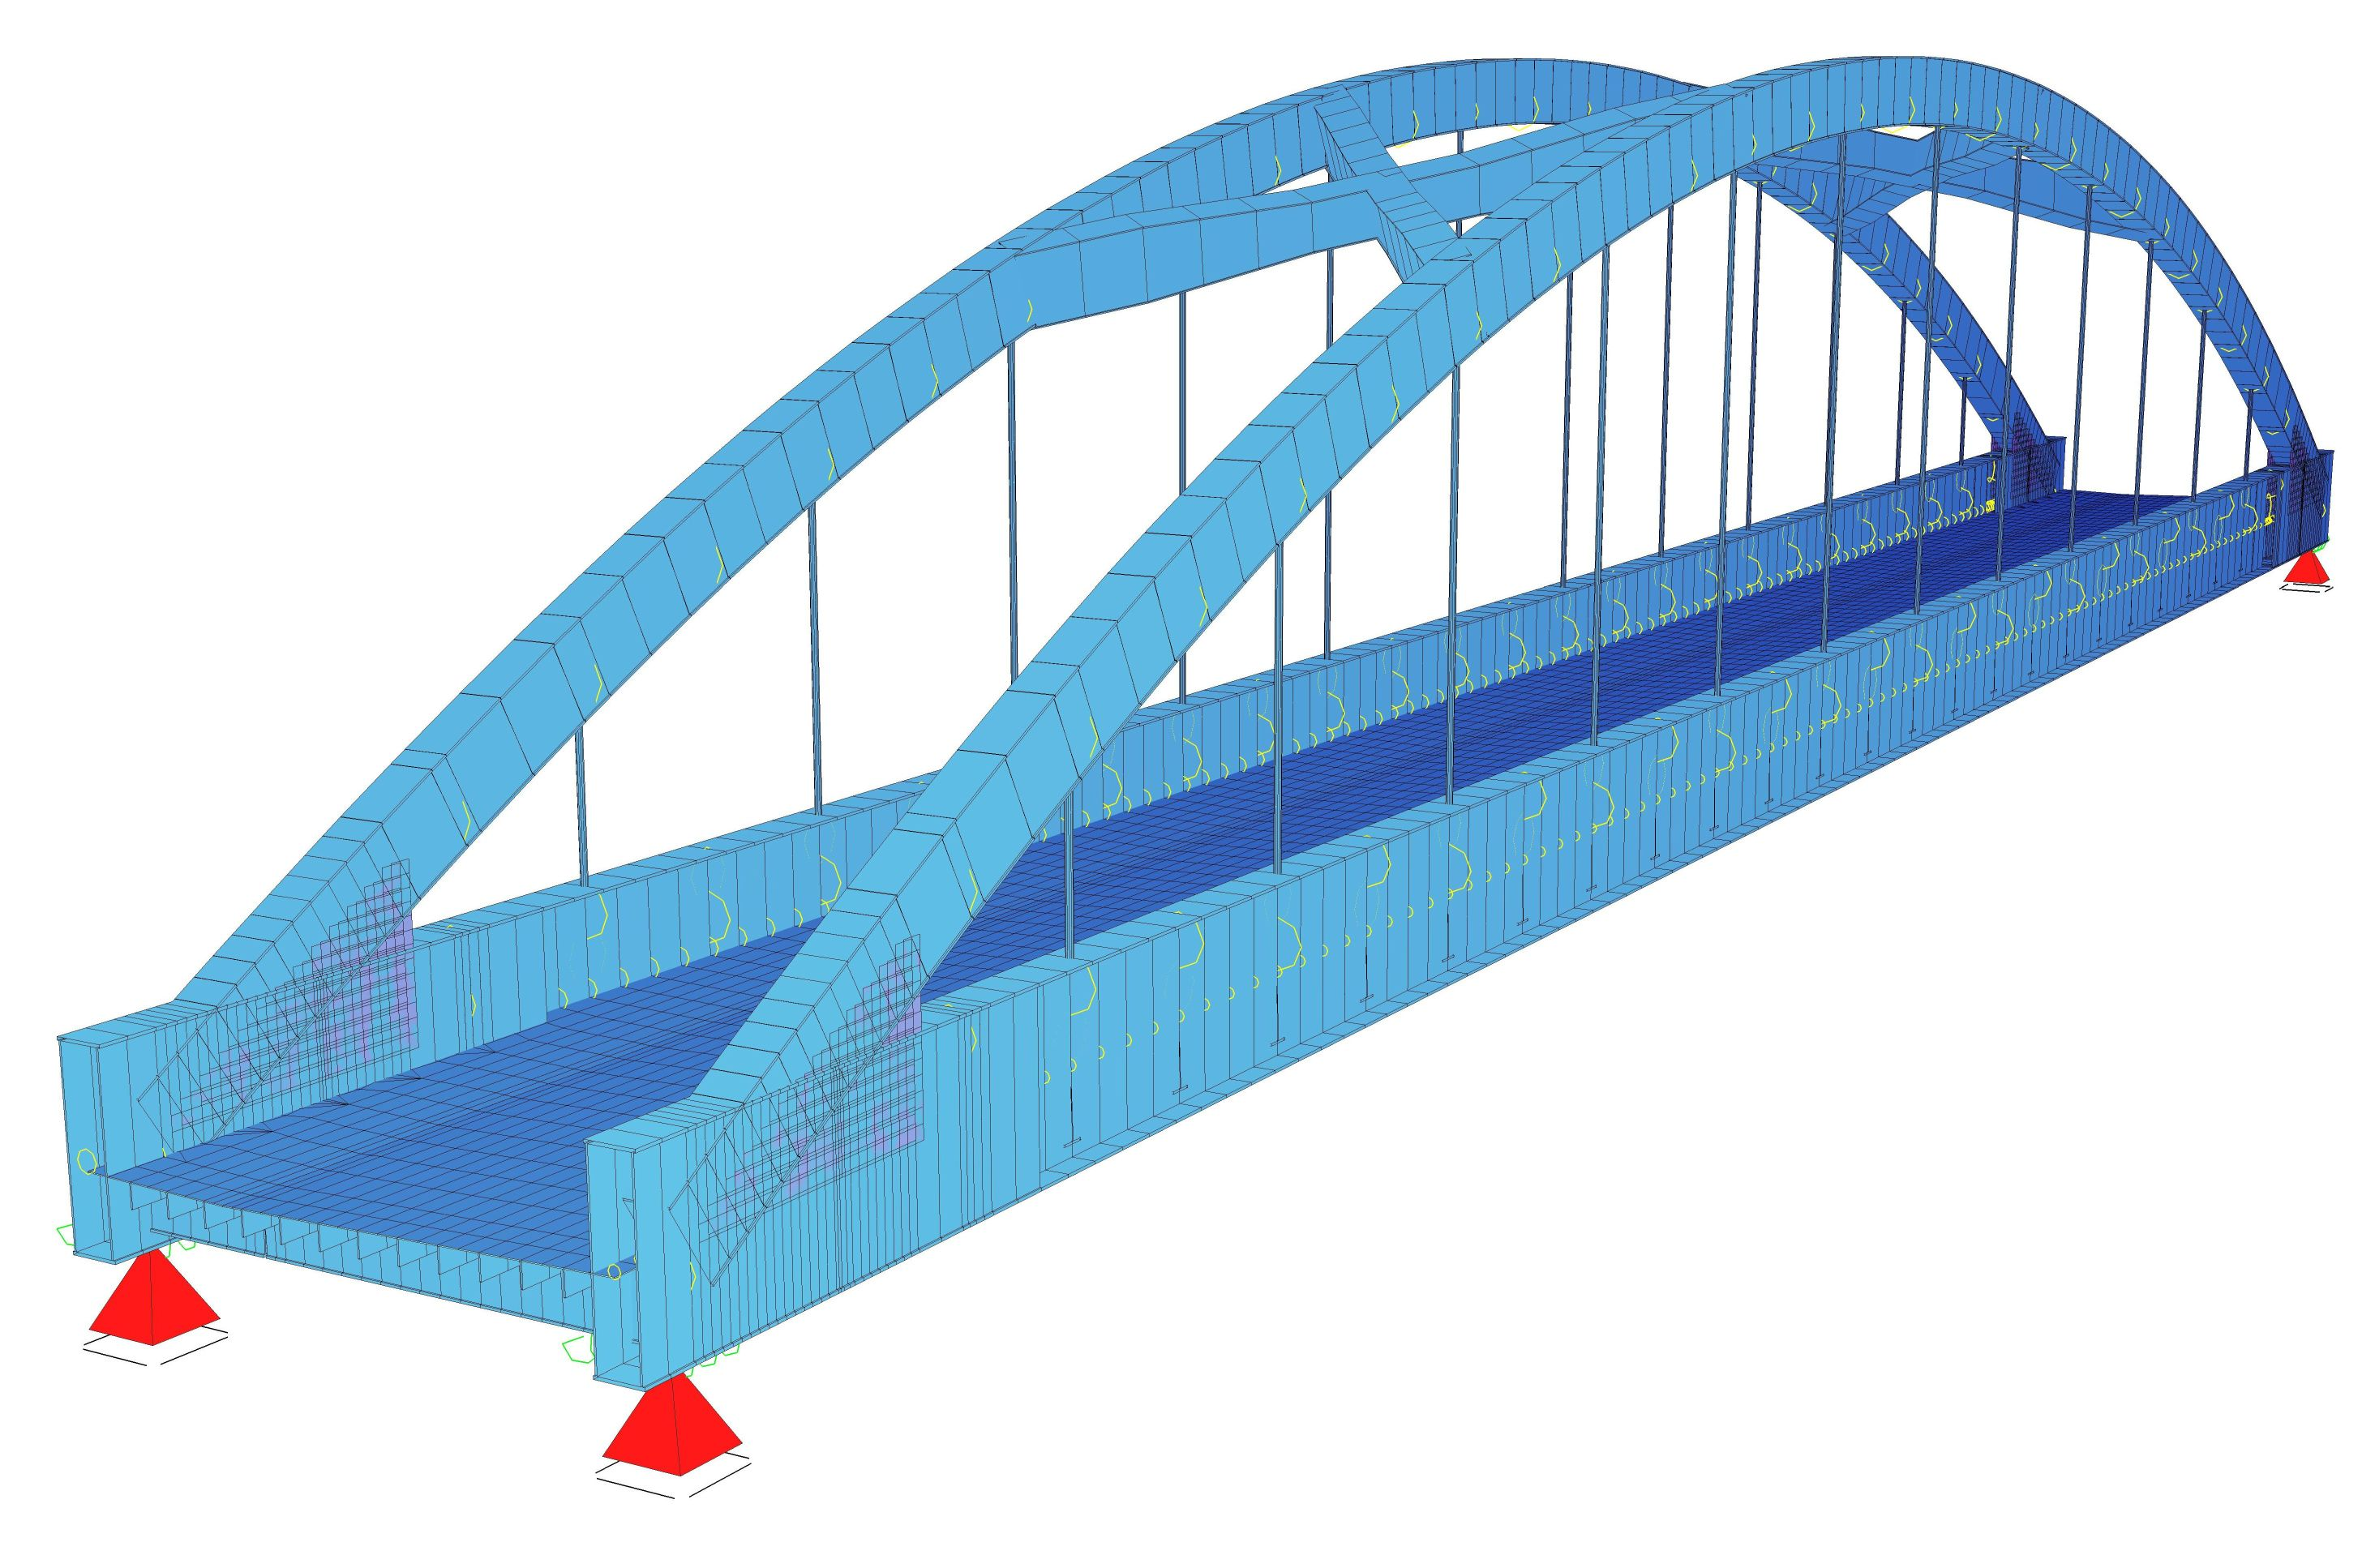
\includegraphics[width=0.5\linewidth]{/WK2/model/SCIAG_PAR_v01_vis_1.jpg}}%
	\subfloat[Widok B]{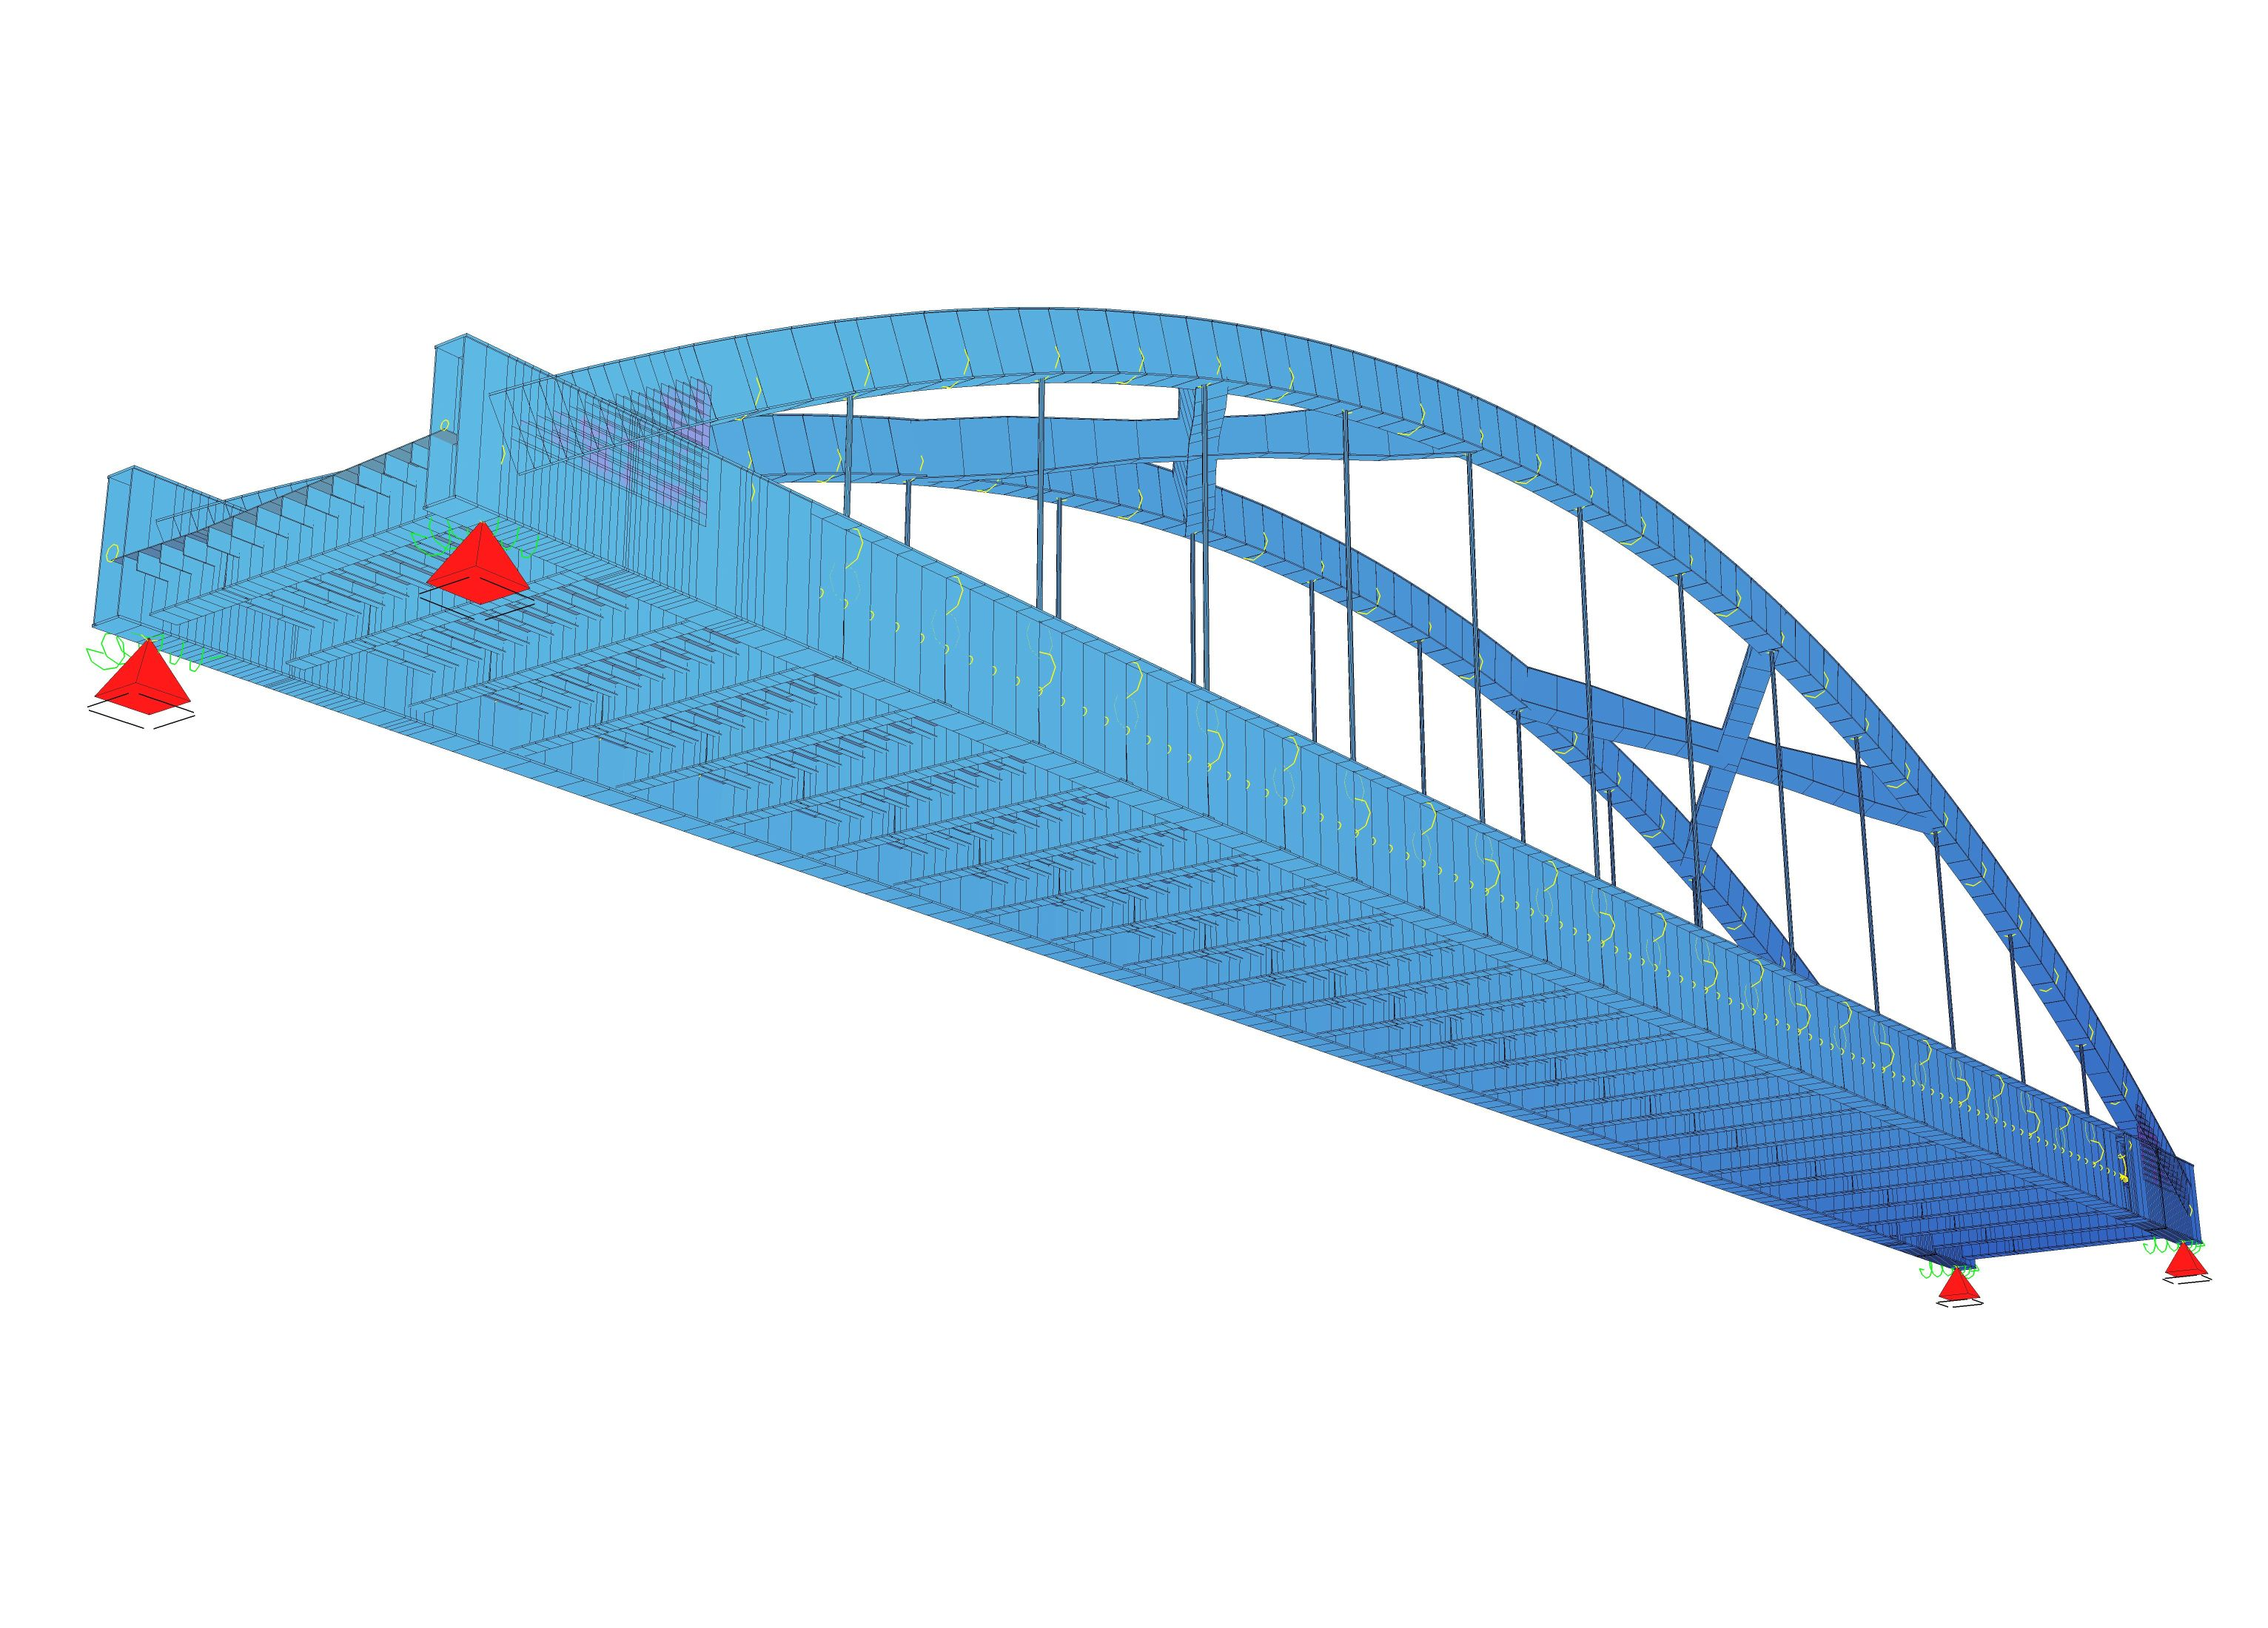
\includegraphics[width=0.5\linewidth]{/WK2/model/SCIAG_PAR_v01_vis_2.jpg}}
	\captionsetup{justification=centering}
	\caption{Wizualizacja przestrzennego modelu numerycznego wiaduktu WK2 Pomorskiej Kolei Metropolitalnej}
	\label{fig: model_wk2_visualization}
\end{figure}
\begin{figure}[h]
	\centering
	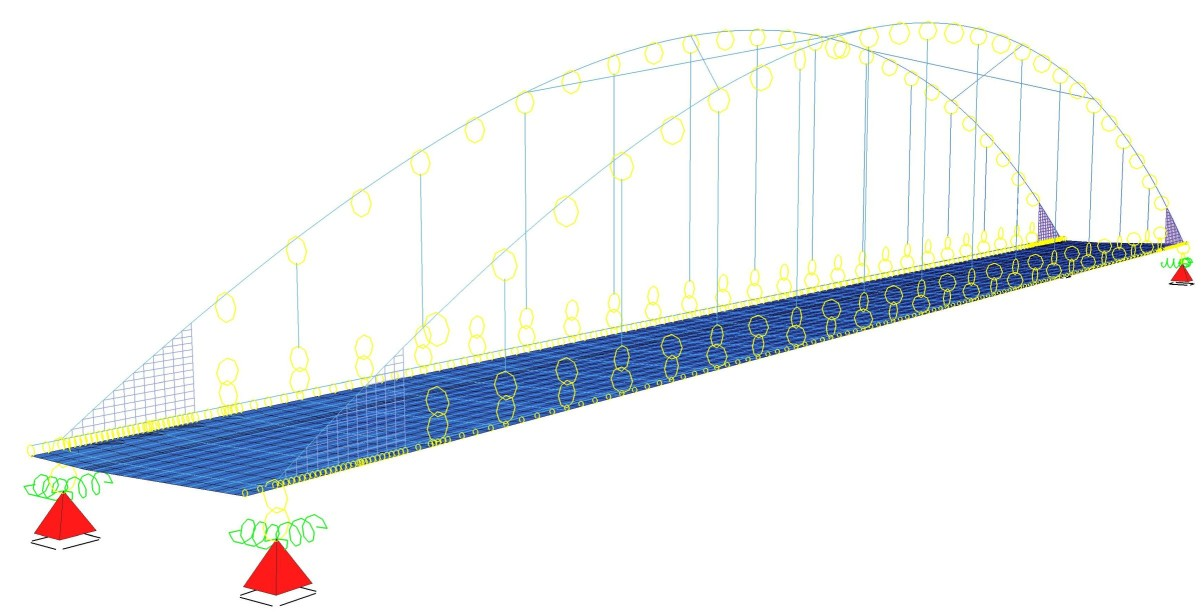
\includegraphics[width=0.8\linewidth]{/WK2/model/SCIAG_PAR_v01_schemat_1.jpg}
	\captionsetup{justification=centering}
	\caption{Schemat statyczny modelu numerycznego wiaduktu WK2 Pomorskiej Kolei Metropolitalnej}
	\label{fig: model_wk2_static_scheme}
\end{figure}

\section{Badania - identyfikacja modalna: wybór punktów, opis badań, wyniki identyfikacji}
Zastosowane kryteria: max mac 0.6, rowno na obie strony, maksymalna srednia z wektorow punktow. Dodac zmiennosc w kombinacjach maksymalnego momentu jako przestroge.
\begin{figure}[h]
	\centering
	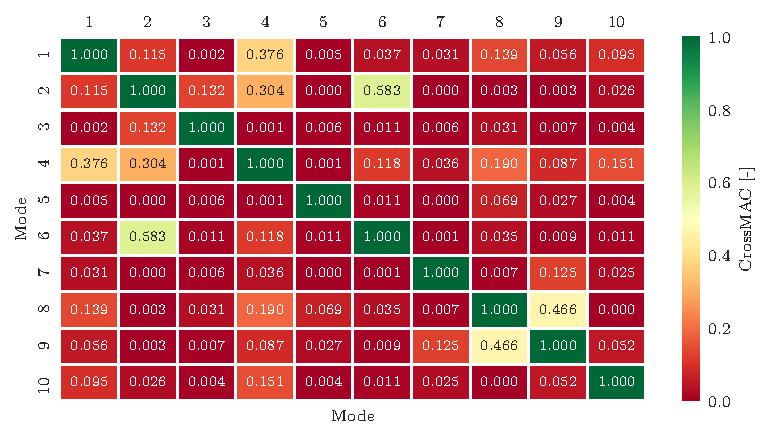
\includegraphics[width=\textwidth]{WK2/correlogram_badania.pdf}
	\captionsetup{justification=centering}
	\caption{Diagram AUTOMAC dla pierwszych dziesięciu wektorów postaci drgań własnych, odczytanych z modelu dla wybranych punktów pomiarowych}
\end{figure}
\begin{figure}[h]
	\centering
	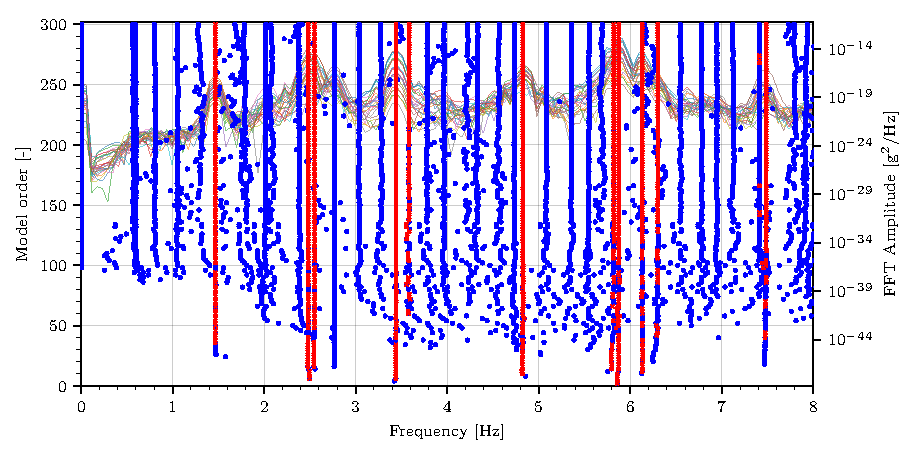
\includegraphics[width=\textwidth]{WK2/diagram_non_filtered.pdf}
	\captionsetup{justification=centering}
	\caption{Diagram stabilizacyjny metody NExT-ERA.}
\end{figure}
\begin{figure}[h]
	\centering
	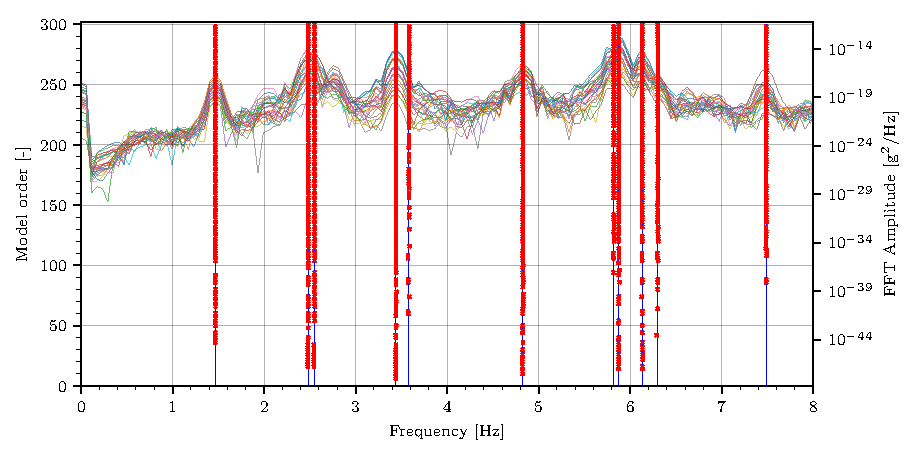
\includegraphics[]{WK2/diagram_filtered2.pdf}
	\captionsetup{justification=centering}
	\caption{Diagram stabilizacyjny metody NExT-ERA.}
\end{figure}
\begin{figure}[h]
	\centering
	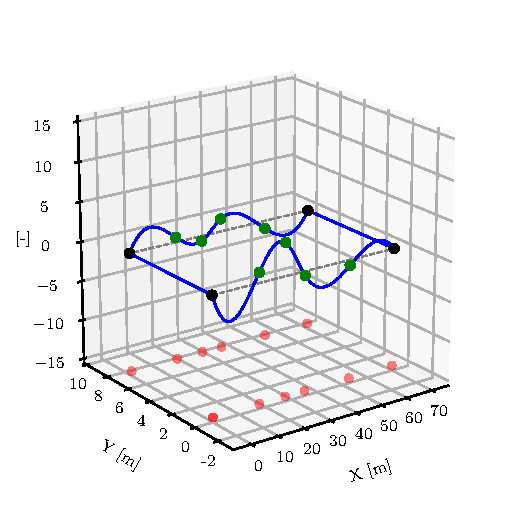
\includegraphics[]{WK2/identified_mode_1.pdf}
	\captionsetup{justification=centering}
	\caption{Diagram stabilizacyjny metody NExT-ERA.}
\end{figure}

\section{Kalibracja modelu numerycznego z wykorzystaniem PSO}
\section{Wielokryterialna optymalizacja modelu: opis + wyniki}
\chapter{Podsumowanie i wnioski}
Podsumowania wnioski